\documentclass[11pt, a4paper]{article}
\usepackage[utf8]{inputenc}
\usepackage[T1]{fontenc}
\usepackage[english]{babel}
\usepackage{geometry}
\usepackage{booktabs}
\usepackage{hyperref}
\usepackage{lmodern}
\usepackage{graphicx}
\usepackage[table]{xcolor} % Ajout pour la couleur des tableaux
\usepackage{pgfplots} % Ajout pour les graphiques
\pgfplotsset{compat=1.18} % Spécifier une version de compatibilité

% Couleurs personnalisées
\definecolor{lightgreen}{rgb}{0.85,1,0.85}
\definecolor{lightorange}{rgb}{1,0.9,0.8}
\definecolor{lightred}{rgb}{1,0.8,0.8}
\definecolor{vuln-critical}{rgb}{0.6,0,0}
\definecolor{vuln-high}{rgb}{1,0.5,0}
\definecolor{vuln-medium}{rgb}{0.8,0.8,0}
\definecolor{vuln-low}{rgb}{0.6,0.8,1}


% Configuration des marges
\geometry{a4paper, margin=1in}

% Configuration des liens hypertextes
\hypersetup{
    colorlinks=true,
    linkcolor=black,
    urlcolor=blue,
    pdftitle={PostgreSQL Security Analysis},
    pdfauthor={Adrien SALES (@rastadidi)},
    pdfsubject={Security, PostgreSQL, Vulnerabilities, DevOps},
    pdfkeywords={PostgreSQL, security, vulnerability, DevOps, DevSecOps, SecOPS, docker, trivy, geol}
}

% Titre et auteur
\title{PostgreSQL Security Analysis\\ \large with \texttt{geol} and \texttt{trivy} tools}
\author{Gemini CLI | Adrien SALES ($\mathbf{X}$ \texttt{@rastadidi})}
\date{\today}

\begin{document}

\maketitle

\begin{abstract}
This article presents a concise analysis of the security and lifecycle of
the \href{https://www.postgresql.org/}{PostgreSQL} database versions.

Using the \href{https://github.com/opt-nc/geol}{\texttt{geol}} tool to check End-of-Life dates and \texttt{trivy} to scan vulnerabilities in official Docker images, I establish a risk profile for currently supported and unsupported versions.\\

The goal is to demonstrate the crucial importance of using maintained versions and the value of combining generative AI with optimally designed CLI tools to automate and enrich this type of analysis.
\end{abstract}

\section{Introduction to the Tools}

Maintaining a secure software infrastructure relies on two fundamental pillars:

\begin{itemize}
    \item \textbf{Actively supported versions}
    \item \textbf{Awareness of vulnerabilities} present in the components we deploy
\end{itemize}

Below is a quick overview of the tools used for this analysis.

\subsection{\texttt{geol}: The Lifecycle Guardian}

\href{https://github.com/opt-nc/geol}{\texttt{geol}} is a tool that queries the \href{https://endoflife.date}{endoflife.date} API to instantly retrieve software End-of-Life dates.

\subsection{\texttt{trivy}: The Vulnerability Scanner}
\href{https://trivy.dev/}{\texttt{trivy}} is an open-source scanner that detects vulnerabilities (CVEs) in container images, file systems, and Git repositories.

\subsection{\texttt{gemini-cli}: AI Assistant}
\href{https://github.com/google-gemini/gemini-cli}{\texttt{gemini-cli}} is an open-source AI agent that brings Gemini's power directly to the terminal.

\subsection{\LaTeX{}: Report Generator}

\LaTeX{} is a document composition system that produces high-quality technical and scientific reports. It is particularly suited for structuring, formatting, and presenting security analysis results clearly and professionally.

\newpage

\section{Data Analysis}

\subsection{Version Lifecycle (\texttt{geol} data)}

The first step is to determine which versions are officially supported.\\

An unsupported version is a \textbf{gateway to unpatched vulnerabilities.}

\begin{table}[h!]
\centering
\caption{PostgreSQL Version Lifecycle}
\label{tab:geol}
\begin{tabular}{@{}lccc@{}}
	
	\textbf{Version} & \textbf{Release Date} & \textbf{End of Support (EOL)} & \textbf{Status} \\ \midrule
\rowcolor{lightgreen} 18 & 2025-09-25 & 2030-11-14 & Supported \\
\rowcolor{lightgreen} 17 & 2024-09-26 & 2029-11-08 & Supported \\
\rowcolor{lightgreen} 16 & 2023-09-14 & 2028-11-09 & Supported \\
\rowcolor{lightgreen} 15 & 2022-10-13 & 2027-11-11 & Supported \\
\rowcolor{lightgreen} 14 & 2021-09-30 & 2026-11-12 & Supported \\
\rowcolor{lightorange} 13 & 2020-09-24 & 2025-11-13 & Approaching End of Life \\ \midrule
\rowcolor{lightred} 12 & 2019-10-03 & 2024-11-21 & \textbf{Unsupported} \\
\rowcolor{lightred} 11 & 2018-10-18 & 2023-11-09 & \textbf{Unsupported} \\
\rowcolor{lightred} 10 & 2017-10-05 & 2022-11-10 & \textbf{Unsupported} \\
\rowcolor{lightred} 9.6 & 2016-09-29 & 2021-11-11 & \textbf{Unsupported} \\ \bottomrule
\end{tabular}
\end{table}


\subsection{Vulnerability Analysis (\texttt{trivy} data)}

The second step is to analyze the "attack surface" of Docker images.

Table \ref{tab:trivy} and Figure \ref{fig:vuln-chart} show the results.

\begin{table}[h!]
\centering
\caption{Vulnerability Summary by Version}
\label{tab:trivy}
\begin{tabular}{@{}lccccc@{}}
	\textbf{Docker Tag} & \textbf{Critical} & \textbf{High} & \textbf{Medium} & \textbf{Low} & \textbf{Total} \\ \midrule
\rowcolor{lightgreen} \texttt{postgres:18} & 0 & 1 & 3 & 97 & 101 \\
\rowcolor{lightgreen} \texttt{postgres:17} & 0 & 1 & 3 & 97 & 101 \\
\rowcolor{lightgreen} \texttt{postgres:16} & 0 & 1 & 3 & 97 & 102 \\
\rowcolor{lightgreen} \texttt{postgres:15} & 0 & 1 & 3 & 97 & 102 \\
\rowcolor{lightgreen} \texttt{postgres:14} & 0 & 1 & 3 & 97 & 102 \\
\rowcolor{lightgreen} \texttt{postgres:13} & 0 & 1 & 3 & 97 & 102 \\ \midrule
\rowcolor{lightorange} \texttt{postgres:12} & 5 & 33 & 56 & 129 & 225 \\
\rowcolor{lightred} \texttt{postgres:11} & 3 & 35 & 12 & 47 & 97 \\
\rowcolor{lightred} \texttt{postgres:10} & 3 & 35 & 12 & 47 & 97 \\
\rowcolor{lightred} \texttt{postgres:9.6} & 6 & 48 & 17 & 47 & 121 \\ \bottomrule
\end{tabular}
\end{table}

\begin{figure}[h!]
\centering
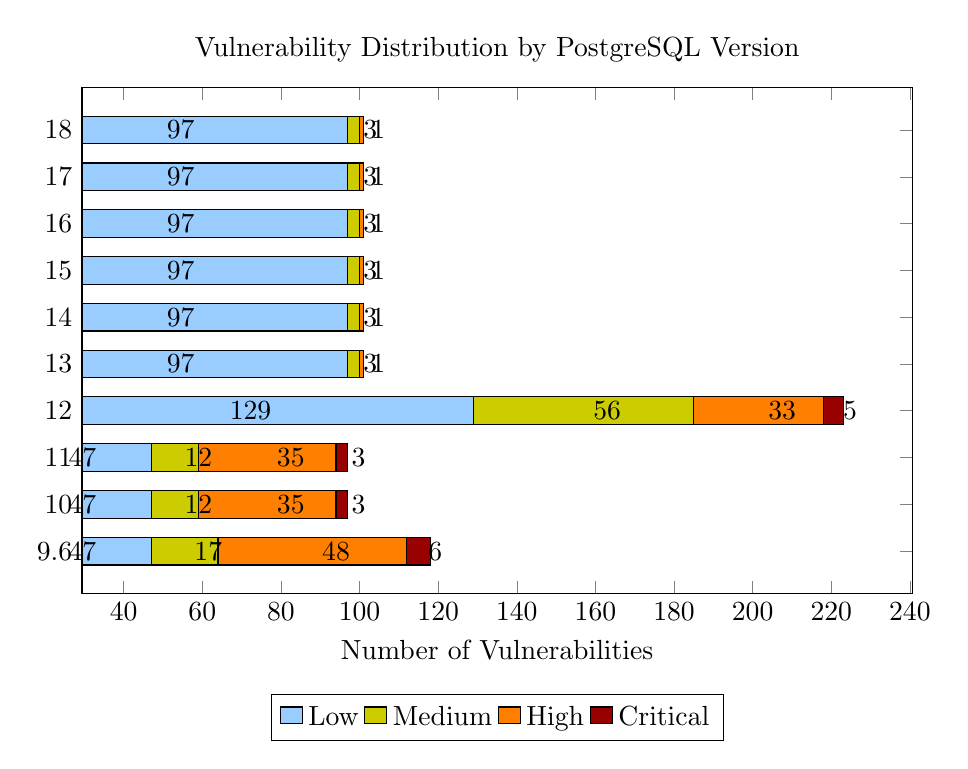
\begin{tikzpicture}
\begin{axis}[
    xbar stacked,
    width=\textwidth,
    height=8cm,
    title={Vulnerability Distribution by PostgreSQL Version},
    xlabel={Number of Vulnerabilities},
    symbolic y coords={9.6, 10, 11, 12, 13, 14, 15, 16, 17, 18},
    ytick=data,
    nodes near coords,
    nodes near coords align={horizontal},
    every node near coords/.style={
        font=\tiny,
        color=black,
        /pgf/number format/precision=0,
        /pgf/number format/fixed,
        /pgf/number format/zerofill=false
    },
    legend style={at={(0.5,-0.2)}, anchor=north, legend columns=-1}
]
\addplot[fill=vuln-low] coordinates {(97,18) (97,17) (97,16) (97,15) (97,14) (97,13) (129,12) (47,11) (47,10) (47,9.6)};
\addplot[fill=vuln-medium] coordinates {(3,18) (3,17) (3,16) (3,15) (3,14) (3,13) (56,12) (12,11) (12,10) (17,9.6)};
\addplot[fill=vuln-high] coordinates {(1,18) (1,17) (1,16) (1,15) (1,14) (1,13) (33,12) (35,11) (35,10) (48,9.6)};
\addplot[fill=vuln-critical] coordinates {(0,18) (0,17) (0,16) (0,15) (0,14) (0,13) (5,12) (3,11) (3,10) (6,9.6)};
\legend{Low, Medium, High, Critical}
\end{axis}
\end{tikzpicture}
\caption{Comparison of vulnerabilities detected by \texttt{trivy}.}
\label{fig:vuln-chart}
\end{figure}


\section{Summary and conclusion}

The combined data analysis is clear. Figure \ref{fig:vuln-chart} strikingly illustrates this divergence:

\begin{itemize}
    \item \textbf{The danger of unsupported versions:} Versions that have reached their end of life (12, 11, 10, 9.6) accumulate a dangerous number of vulnerabilities, including several \textbf{critical} ones.
    \item \textbf{The security of supported versions:} In contrast, images of maintained versions (13 to 18) show no critical vulnerabilities and a low, consistent risk profile. Note that PostgreSQL 13 will reach EOL soon (2025-11-13).
    \item \textbf{Recommendation:} The choice of PostgreSQL version must be for an actively supported version. The security risk of using an obsolete version is real and high.\\
\end{itemize}

Tools like \texttt{geol} and \texttt{trivy} are essential in a modern DevSecOps approach. This analysis of PostgreSQL perfectly illustrates how abandoning software support directly leads to a drastic increase in security flaws. Using up-to-date versions is not just a recommendation, but a necessity for the security of any infrastructure.

\end{document}
